% Options for packages loaded elsewhere
\PassOptionsToPackage{unicode}{hyperref}
\PassOptionsToPackage{hyphens}{url}
\documentclass[
]{article}
\usepackage{xcolor}
\usepackage{amsmath,amssymb}
\setcounter{secnumdepth}{-\maxdimen} % remove section numbering
\usepackage{iftex}
\ifPDFTeX
  \usepackage[T1]{fontenc}
  \usepackage[utf8]{inputenc}
  \usepackage{textcomp} % provide euro and other symbols
\else % if luatex or xetex
  \usepackage{unicode-math} % this also loads fontspec
  \defaultfontfeatures{Scale=MatchLowercase}
  \defaultfontfeatures[\rmfamily]{Ligatures=TeX,Scale=1}
\fi
\usepackage{lmodern}
\ifPDFTeX\else
  % xetex/luatex font selection
\fi
% Use upquote if available, for straight quotes in verbatim environments
\IfFileExists{upquote.sty}{\usepackage{upquote}}{}
\IfFileExists{microtype.sty}{% use microtype if available
  \usepackage[]{microtype}
  \UseMicrotypeSet[protrusion]{basicmath} % disable protrusion for tt fonts
}{}
\makeatletter
\@ifundefined{KOMAClassName}{% if non-KOMA class
  \IfFileExists{parskip.sty}{%
    \usepackage{parskip}
  }{% else
    \setlength{\parindent}{0pt}
    \setlength{\parskip}{6pt plus 2pt minus 1pt}}
}{% if KOMA class
  \KOMAoptions{parskip=half}}
\makeatother
\usepackage{longtable,booktabs,array}
\usepackage{calc} % for calculating minipage widths
% Correct order of tables after \paragraph or \subparagraph
\usepackage{graphicx}
\graphicspath{{C:/Users/juanf/OneDrive/Documentos/GitHub/EnergyScope_coupling_GEMMES/Docs/}}
\usepackage{etoolbox}
\makeatletter
\patchcmd\longtable{\par}{\if@noskipsec\mbox{}\fi\par}{}{}
\makeatother
% Allow footnotes in longtable head/foot
\IfFileExists{footnotehyper.sty}{\usepackage{footnotehyper}}{\usepackage{footnote}}
\makesavenoteenv{longtable}
\usepackage{graphicx}
\makeatletter
\newsavebox\pandoc@box
\newcommand*\pandocbounded[1]{% scales image to fit in text height/width
  \sbox\pandoc@box{#1}%
  \Gscale@div\@tempa{\textheight}{\dimexpr\ht\pandoc@box+\dp\pandoc@box\relax}%
  \Gscale@div\@tempb{\linewidth}{\wd\pandoc@box}%
  \ifdim\@tempb\p@<\@tempa\p@\let\@tempa\@tempb\fi% select the smaller of both
  \ifdim\@tempa\p@<\p@\scalebox{\@tempa}{\usebox\pandoc@box}%
  \else\usebox{\pandoc@box}%
  \fi%
}
% Set default figure placement to htbp
\def\fps@figure{htbp}
\makeatother
\setlength{\emergencystretch}{3em} % prevent overfull lines
\providecommand{\tightlist}{%
  \setlength{\itemsep}{0pt}\setlength{\parskip}{0pt}}
\usepackage{bookmark}
\IfFileExists{xurl.sty}{\usepackage{xurl}}{} % add URL line breaks if available
\urlstyle{same}
\hypersetup{
  pdftitle={Model formulation},
  hidelinks,
  pdfcreator={LaTeX via pandoc}}

\title{Model formulation}
\author{}
\date{}

\begin{document}
\maketitle

\textbf{Model overview:}

\begin{figure}
\centering
\pandocbounded{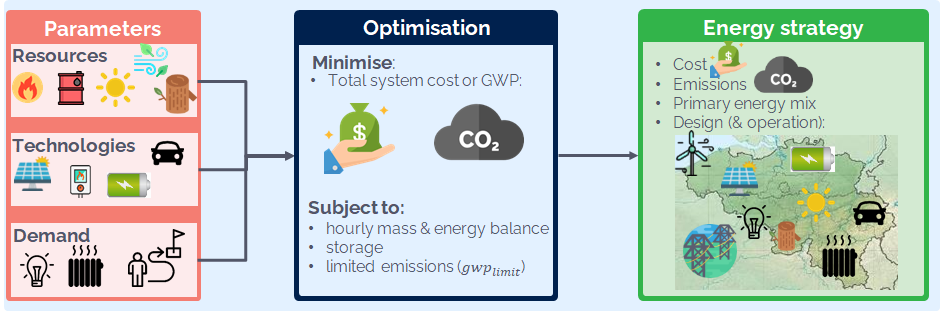
\includegraphics[keepaspectratio]{/images/model_formulation/chp_estd_overview.png}}
\caption{Overview of the LP modelling framework.}
\end{figure}

\section{Overview}\label{overview}

Due to computational restrictions, energy system models rarely optimise
over the 8760 hours of the year. For example, running our model with
8760h time series takes more than 19 hours, while it takes only around 1
minute with the methodology presented hereafter.

A typical solution is to use a subset of Typical (i.e. representative)
Days called TD; this is a trade-off between introducing an approximation
error in the representation of the energy system (especially for
short-term dynamics) and computational time.

Running the EnergyScope Typical Day (ESTD) model consists in two steps:

\begin{itemize}
\tightlist
\item
  the first step consists in pre-processing the time series and solving  a MILP problem to determine the adequate set of typical days   (\texttt{sec\_td\_selection}).
\item
  the second step is the main energy model: the optimal design and
  operation of the energy system over the selected typical days is
  computed i.e.~technology selection, sizing and operation for a target
  future year (\texttt{sec\_estd})
\end{itemize}

These two steps can be performed independently. Usually, the first step
is computed only once for an energy system with given weather data
whereas the second step is computed several times (once for each
different scenario).
\texttt{Figure\ \%s\ \textless{}fig:ProcessStructure\textgreater{}}
illustrates the overall structure of the code.

\begin{figure}
\centering
\pandocbounded{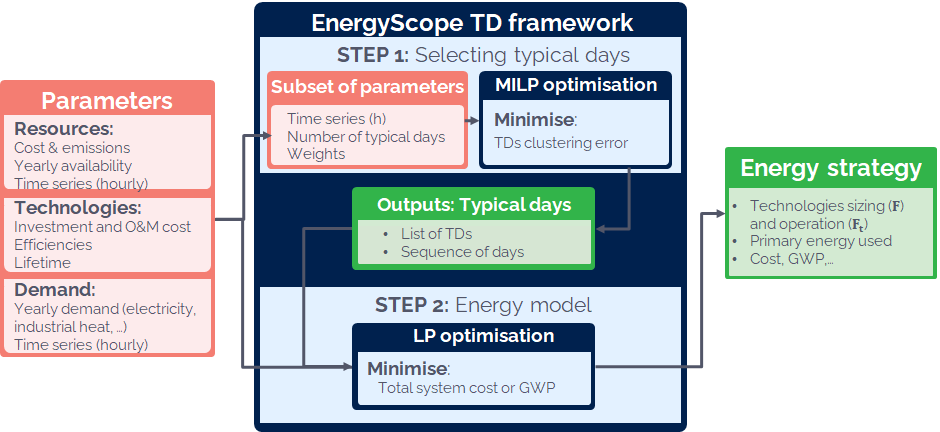
\includegraphics[keepaspectratio]{/images/model_formulation/meth_process_structure.png}}
\caption{Overview of the EnergyScope TD framework in two-steps.
\textbf{STEP 1}: optimal selection of typical days
(\texttt{sec\_td\_selection}). \textbf{STEP 2}: Energy system model
(\texttt{sec\_estd}). The first step processes only a subset of
parameters, which account for the 8760h time series. Abbreviations:
Typical Day (TD), Linear Programming (LP), Mixed Integer Linear
Programming (MILP), Global Warming Potential (GWP).}
\end{figure}

This documentation is built based on previous works
Moret2017PhDThesis,Limpens2019,Limpens2021thesis. For more details about
the research approach, the choice of clustering method or the
reconstruction method, see Limpens2021thesis.

\section{Typical days selection}\label{sec_td_selection}

Resorting to TDs has the main advantage of reducing the computational
time by several orders of magnitude. Usually, studies use between 6 and
20 TDs Gabrielli2018,Despres2017,Nahmmacher2014,Pina2013 and sometimes
even less Poncelet2017,Dominguez-Munoz2011.

\subsection{Clustering methods}\label{clustering-methods}

In a previous work Limpens2019, it has been estimated that 12 typical
days were appropriate for this model. Moreover, a comparison between
different clustering algorithms showed that the method of
Dominguez-Munoz2011 had the best performances.

\subsection{Implementing seasonality with typical
days}\label{implementing-seasonality-with-typical-days}

Using TDs can introduce some limitations. For example, model based on
TDs are traditionally not able to include inter-days or seasonal storage
due to the discontinuity between the selected days. Thus, they assess
only the capacity of production without accounting for storage
capacities. Carbon-neutral energy system will require long term storage
and thus, this limitation had to be overcome. Therefore, we implemented
a method proposed by Gabrielli2018 to rebuild a year by defining it as a
sequence of typical days. This allows to optimise the storage level of
charge over the 8760 hours of the year. Gabrielli2018 assigned a TD to
each day of the year; all decision variables are optimised over the TDs,
apart from the amount of energy stored, which is optimised over 8760
hours. This methodology is illustrated in
\texttt{Figure\ \%s\ \textless{}fig:SeasonalityImplementation\textgreater{}}.

\begin{figure}
\centering
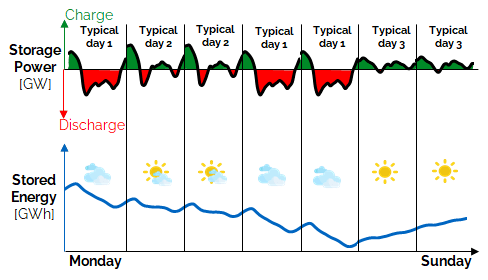
\includegraphics[width=14cm,height=\textheight,keepaspectratio]{/images/model_formulation/gabrielli.png}
\caption{Illustration of the typical days reconstruction method proposed
by Gabrielli2018 over a week. The example is based on 3 TDs: TD 1
represents a cloudy weekday, applied to Monday, Thursday and Friday; TD
2 is a sunny weekday, applied to Tuesday and Wednesday; finally, TD 3
represents sunny weekend days. The power profile (above) depends solely
on the typical day but the energy stored (below) is optimised over the
8760 hours of the year (blue curve). Note that the level of charge is
not the same at the beginning (Monday 1 a.m.) and at the end of the week
(Sunday 12 p.m.).}
\end{figure}

The performances of this method have been quantified in a previous work
Limpens2019. With 12 typical days, the key performance indicators (cost,
emissions, installed capacity and primary energy used) are well
captured. The only exception are the long term storage capacities, which
are slightly underestimated (by a factor of 2 at most).

\section{Energy system model}\label{sec_estd}

In this section, we present the core of the energy model. First, we
introduce the conceptual modelling framework with an illustrative
example. This helps to clarify the nomenclature as well. Second, we
introduce the constraints of the optimization problem. The data used in
the model, on the other hand, are detailed in the sections
\texttt{/sections/Input\ Data\ -\ Colombia} and
\texttt{/sections/Input\ Data\ -\ Turkey}.

\subsection{Linear programming formulation}\label{ssec_lp_framework}

The model is mathematically formulated as a LP problem
fourer1990modeling.
\texttt{Figure\ \%s\ \textless{}fig:linear\_programming\_example\textgreater{}}
represents - in a simple manner - what is a LP problem and the related
nomenclature. In italic capital letters, \emph{SETS} are collections of
distinct items. For example, the \emph{RESOURCES} set regroups all the
available resources (NG, WOOD, etc.). In italic lowercase letters,
\emph{parameters} are known values (inputs) of the model, such as
specific end-use demands and resource availabilities. In bold with first
letter in uppercase, \textbf{Variables} are unknown values of the model,
such as the installed capacity of PV. These values are determined (i.e.
optimised) by the solver within an upper and a lower bound (both being
parameters). For example, the installed capacity of wind turbines is a
\emph{decision variable}. This quantity is bounded between zero and the
maximum available wind potential. \emph{Decision variables} can be split
in two categories: independent decision variables, which can be freely
fixed, and dependent decision variables, which are linked via equality
constraints to the previous ones. For example, the investment cost for
wind turbines is a variable but it directly depends on the installed
capacity of wind turbines, which is an independent decision variable.
\emph{Constraints} are inequality or equality that must be satisfied
between variables parameters. The problem is subject to (\emph{s.t.})
constraints that can enforce, for example, an energy balance or an upper
limit for the availability of resources. Finally, an \emph{objective
function} is a particular variable whose value is to be minimised (or
maximised).

\begin{figure}
\centering
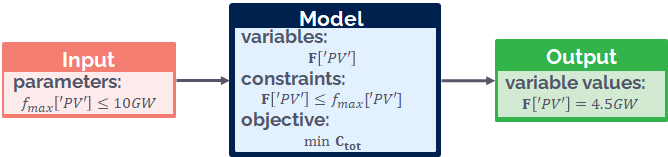
\includegraphics[width=14cm,height=\textheight,keepaspectratio]{/images/model_formulation/chp_estd_lp_conceptual.png}
\caption{Conceptual illustration of a LP problem, with the related
nomenclature. Description of symbols: maximum installable capacity for a
technology (f \textsubscript{max}), installed capacity of a technology
(\textbf{F}) and total system cost (\textbf{C\_tot}). In this example, a
specific technology (\textbf{F} {[}\emph{'PV'}{]}) has been chosen from
the set TECHNOLOGY.}
\end{figure}

\subsection{Conceptual modelling
framework}\label{app:sec:conceptual_modelling_framework}

The proposed modelling framework is a simplified representation of an
energy system, accounting for the energy flows within its boundaries.
Its primary objective is to satisfy the energy balance constraints,
meaning that the demand is given and the supply has to meet it. In
energy modelling practice, the energy demand is often expressed in terms
of Final Energy Consumption (FEC). According to the definition of the
European commission, FEC is defined as ``\emph{the energy which reaches
the final consumer's door}'' EU\_FEC. In other words, the FEC is the
amount of input energy needed to satisfy the end-use demand (EUD). For
example, in the case of decentralised heat production with a natural gas
boiler, the FEC is the amount of natural gas consumed by the boiler,
while the EUD is the amount of heat produced by the boiler i.e.~the heat
delivered to the user.

The input of the proposed modelling framework here is not the FEC but
the EUD, related to five energy sectors: electricity, heating, cooling,
mobility and non-energy. This replaces the classical economic-sector
based representation of energy demand. Heat is divided in three end-use
types (EUT): high temperature heat for industry, low temperature heat
for space heating and low temperature heat for hot water. Cooling is
divided in two EUTs: process cooling (for industry) and space cooling.
Mobility is divided in two EUTs: passenger mobility and
freight\footnote{Air passenger transport is accounted for in passenger
  mobility (excluding international flights).}. Non-energy demand is,
based on the IEA definition, ``\emph{fuels that are used as raw
materials in the different sectors and are not consumed as a fuel or
transformed into another fuel.}'' IEA\_websiteDefinition. For example,
the European Commission classifies as non-energy the following
materials: ``\emph{chemical feed-stocks, lubricants and asphalt for road
construction.}'' EuropeanCommission2016.

\begin{figure}
\centering
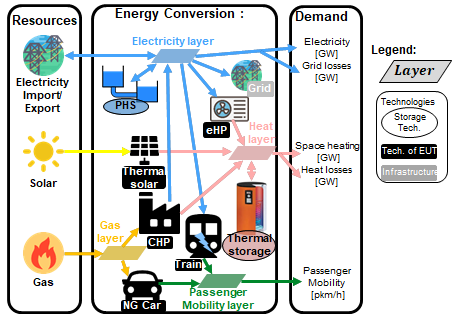
\includegraphics[width=16cm,height=\textheight,keepaspectratio]{/images/model_formulation/chp_estd_conceptual_framework.png}
\caption{Conceptual example of an energy system with 3 resources, 3 EUDs
and 8 technologies, among which 2 of storage type (coloured oval) and 1
of infrastructure type (grey rectangle). Abbreviations: pumped hydro
storage (PHS), electrical heat pump (eHP), cogenerations of heat and
power (CHP), natural gas (NG). Some icons from FlatIcon.}
\end{figure}

A simplified conceptual example of the energy system\textquotesingle s
structure is proposed in
\texttt{Figure\ \%s\ \textless{}fig:conceptual\_example\textgreater{}}.
The system is split in three parts: resources, energy conversion and
demand. In this illustrative example, resources are solar energy,
electricity and natural gas (NG). The EUDs are demands for electricity,
space heating and passenger mobility. The energy system encompasses all
the energy conversion technologies needed to transform resources in
order to fulfill the EUD. In this example, solar and NG resources cannot
be directly used to supply heat. Thus, technologies are used, such as
boilers or cogenerations of heat and power (CHP) using NG, to supply the
EUT layers (in this case, the \emph{high-temperature heat for industry}
layer). \emph{Layers} are defined as all the elements in the system that
need to be balanced in each time period; they include resources and
EUTs. For example, the electricity layer must be balanced at any time,
meaning that the production and storage must equal the consumption and
losses. These layers are connected to one another by
\emph{technologies}. We define three types of technologies:
\emph{technologies of end-use type}, \emph{storage technologies} and
\emph{infrastructure technologies}. A technology of end-use type can
convert the energy (e.g. a fuel resource) from one layer to an EUT
layer, such as a CHP unit that converts NG into heat and electricity. A
storage technology converts energy from a layer to the same one, such as
thermal storage (TS) that stores heat to provide heat. In our example
(\texttt{Figure\ \%s\ \textless{}fig:conceptual\_example\textgreater{}}),
there are two storage technologies: TS for heat and pumped hydro storage
(PHS) for electricity. Infrastructure technologies include all the
remaining technologies, including the networks, such as the power grid
and district heating networks (DHN), but also technologies linking non
end-use layers, such as methane production from wood gasification or
hydrogen production from methane reforming.

As an illustrative example of the concept of \emph{layer},
\texttt{Figure\ \%s\ \textless{}fig:LayerElec\textgreater{}} presents a
sketch of the electricity layer, which is the most complex one since the
electrification of other sectors is foreseen as a key element of the
energy transition Sugiyama2012. In the version of EnergyScope described
in this document, 54 technologies are related to the electricity layer.
16 technologies produce electricity exclusively, such as combined cycle
gas turbine (CCGT), rooftop PV or onshore wind. 14 cogenerations of heat
and power (CHPs) produce both heat and electricity, such as industrial
waste CHP. 10 technologies are related to the production of synthetic
fuels and to carbon capture and storage (CCS). 1 infrastructure
technology represents the electrical grid. 6 storage technologies are
implemented, such as PHS, batteries or vehicle-to-grid (V2G). The rest
relates to the electrification of heat and mobility. Electrification of
the heating sector is supported by direct electric heating and, most
importantly, by electrical heat pumps. Electrification of mobility is
achieved via electric public transportation (train, trolley, metro and
electrical/hybrid bus), electric private transportation including
battery and hydrogen cars\footnote{Hydrogen can be produced based on
  many feedstocks, among which electricity via the use of electrolysers.}
and electric freight with trains.

\begin{figure}
\centering
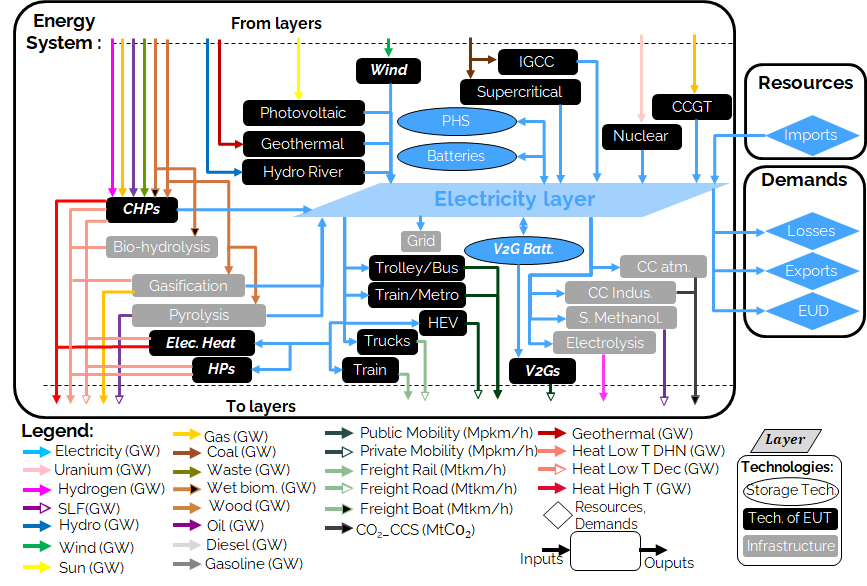
\includegraphics[width=16cm,height=\textheight,keepaspectratio]{/images/model_formulation/Layer_Elec.png}
\caption{Representation of the \emph{electricity} layer with all the
technologies implemented in ESTD v2.1. (The version descripted in this
document is v2.2.) Bold italic technologies represent a group of
different technologies. Abbreviations: electricity (elec.), industrial
(ind.), combined cycle gas turbine (CCGT), integrated gasification
combined cycle with coal (IGCC), cogeneration of heat and power (CHP),
heat pump (HP), pumped hydro storage (PHS), vehicle-to-grid (V2G),
synthetic methanolation (S. Methanol.), atmospheric (atm.), carbon
capture (CC), end-use demand (EUD).}
\end{figure}

The model is formulated as a LP problem. It optimises the design of the
energy system by computing the installed capacity of each technology, as
well as the operation in each period, that minimizes the total annual
cost of the system while meeting the energy demand. In the following
sections, we present the complete formulation of the model in two steps.
First, all the terms used are summarised in a figure and a set of tables
(\texttt{Figure\ \%s\ \textless{}fig:sets\textgreater{}} for sets,
Tables \texttt{\%s\ \textless{}tab:paramsDistributions\textgreater{}}
and \texttt{\%s\ \textless{}tab:params\textgreater{}} for parameters,
Tables \texttt{\%s\ \textless{}tab:variablesIndependent\textgreater{}}
and \texttt{\%s\ \textless{}tab:variablesdependent\textgreater{}} for
variables). Second, on this basis, the equations representing the
constraints and the objective function are presented in
\texttt{Figure\ \%s\ \textless{}fig:EndUseDemand\textgreater{}} and
detailed in Eqs.~\texttt{eq:obj\_func} - \texttt{eq:efficiency}.

\subsection{Sets, parameters and variables}\label{ssec_sets_params_vars}

\texttt{Figure\ \%s\ \textless{}fig:sets\textgreater{}} gives a visual
representation of the sets used in EnergyScope, together with their
respective indices. Tables
\texttt{\%s\ \textless{}tab:paramsDistributions\textgreater{}} and
\texttt{\%s\ \textless{}tab:params\textgreater{}} list and describe the
model parameters. Tables
\texttt{\%s\ \textless{}tab:variablesIndependent\textgreater{}} and
\texttt{\%s\ \textless{}tab:variablesdependent\textgreater{}} list and
describe the independent and dependent variables, respectively.

\begin{figure}
\centering
\pandocbounded{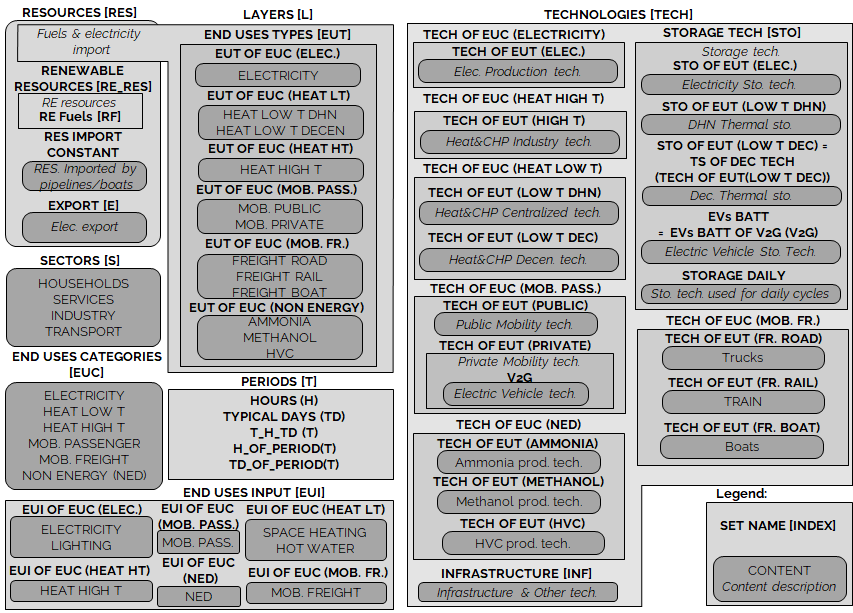
\includegraphics[keepaspectratio]{/images/model_formulation/ses_sets_v2.png}}
\caption{Visual representation of the sets and indices used in the LP
framework. This figure was produced for ESTD v2.1 and does not include
the latest technologies and EUDs included in v2.2, such as the ones
related to cooling. Abbreviations: space heating (SH), heating water
(HW), temperature (T), mobility (MOB), passenger (\emph{Pass.}),
vehicle-to-grid (V2G), thermal storage (TS).}
\end{figure}

\begin{longtable}[]{@{}
  >{\raggedright\arraybackslash}p{(\linewidth - 4\tabcolsep) * \real{0.3889}}
  >{\raggedright\arraybackslash}p{(\linewidth - 4\tabcolsep) * \real{0.1667}}
  >{\raggedright\arraybackslash}p{(\linewidth - 4\tabcolsep) * \real{0.3889}}@{}}
\caption{Exhaustive list of time series parameters used in ESTD
v2.2.}\tabularnewline
\toprule\noalign{}
\begin{minipage}[b]{\linewidth}\raggedright
\textbf{Parameter}
\end{minipage} & \begin{minipage}[b]{\linewidth}\raggedright
\textbf{Units}
\end{minipage} & \begin{minipage}[b]{\linewidth}\raggedright
\textbf{Description}
\end{minipage} \\
\midrule\noalign{}
\endfirsthead
\toprule\noalign{}
\begin{minipage}[b]{\linewidth}\raggedright
\textbf{Parameter}
\end{minipage} & \begin{minipage}[b]{\linewidth}\raggedright
\textbf{Units}
\end{minipage} & \begin{minipage}[b]{\linewidth}\raggedright
\textbf{Description}
\end{minipage} \\
\midrule\noalign{}
\endhead
\bottomrule\noalign{}
\endlastfoot
\(\%_{elec}(h,td)\) & {[}-{]} & Yearly time series (adding up to 1) of
electricity EUD \\
\(\%_{sh}(h,td)\) & {[}-{]} & Yearly time series (adding up to 1) of
space heating EUD \\
\(\%_{sc}(h,td)\) & {[}-{]} & Yearly time series (adding up to 1) of
space cooling EUD \\
\(\%_{pass}(h,td)\) & {[}-{]} & Yearly time series (adding up to 1) of
passenger mobility EUD \\
\(\%_{fr}(h,td)\) & {[}-{]} & Yearly time series (adding up to 1) of
freight mobility EUD \\
\(c_{p,t}(tech,h,td)\) & {[}-{]} & Hourly maximum capacity factor for
each technology (default 1) \\
\end{longtable}

\begin{longtable}[]{@{}
  >{\raggedright\arraybackslash}p{(\linewidth - 4\tabcolsep) * \real{0.3194}}
  >{\raggedright\arraybackslash}p{(\linewidth - 4\tabcolsep) * \real{0.3194}}
  >{\raggedright\arraybackslash}p{(\linewidth - 4\tabcolsep) * \real{0.3194}}@{}}
\caption{Exhaustive list of parameters (except time series) used in ESTD
v2.2.}\tabularnewline
\toprule\noalign{}
\begin{minipage}[b]{\linewidth}\raggedright
Parameter
\end{minipage} & \begin{minipage}[b]{\linewidth}\raggedright
Units
\end{minipage} & \begin{minipage}[b]{\linewidth}\raggedright
Description
\end{minipage} \\
\midrule\noalign{}
\endfirsthead
\toprule\noalign{}
\begin{minipage}[b]{\linewidth}\raggedright
Parameter
\end{minipage} & \begin{minipage}[b]{\linewidth}\raggedright
Units
\end{minipage} & \begin{minipage}[b]{\linewidth}\raggedright
Description
\end{minipage} \\
\midrule\noalign{}
\endhead
\bottomrule\noalign{}
\endlastfoot
\(\tau\)(tech) & {[}-{]} & Investment cost annualization factor \\
\(i_{rate}\) & {[}-{]} & Real discount rate \\
\(endUses_
{year} (eui,s)\) & {[}GWh/y{]} \hyperref[a]{{[}a{]}} & Annual EUD values
divided per sector \\
\(endUsesInput
(eui)\) & {[}GWh/y{]} \hyperref[a]{{[}a{]}} & Total annual EUD values \\
\(re_{share}\) & {[}-{]} & Minimum share {[}0;1{]} of primary energy
coming from renewables \\
\(gwp
_{limit}\) & {[}ktCO\(_{2}\)-eq/y{]} & Upper CO\(_{2}\)-eq emissions
limit \\
\(\%_
{public,min},
\%_{public,max}\) & {[}-{]} & Lower and upper limit to \(\textbf{\%}_
{\textbf{Public}}\) \\
\(\%_
{fr,rail,min},
\%_{fr,rail,max}\) & {[}-{]} & Lower and upper limit to \(\textbf{\%}_
{\textbf{Fr,Rail}}\) \\
\(\%_
{fr,boat,min},
\%_{fr,boat,max}\) & {[}-{]} & Lower and upper limit to \(\textbf{\%}_
{\textbf{Fr,Boat}}\) \\
\(\%_
{fr,truck,min},
\%_{fr,truck,max}\) & {[}-{]} & Lower and upper limit to \(\textbf{\%}_
{\textbf{Fr,Truck}}\) \\
\(\%_
{private,motorc,max}\) & {[}-{]} & Max. share of private mobility
supplied by motorcycles \\
\(\%_
{dhn,min},
\%_{dhn,max}\) & {[}-{]} & Lower and upper limit to \(\textbf{\%}_
{\textbf{Dhn}}\) \\
\(\%_
{ned}(EUT\_OF\_EUC(
NON\_ENERGY))\) & {[}-{]} & Share of non-energy demand per type of
feedstock \\
\(t_
{op}(h,td)\) & {[}h{]} & Duration of each time period (default 1h) \\
\(f_{min},
f_{max}
(tech)\) & {[}GW{]} \hyperref[a]{{[}a{]}} \hyperref[b]{{[}b{]}} &
Min./max. installed size of each technology \\
\(f_{min,\%},
f_{max,\%}(tech)\) & {[}-{]} & Min./max. relative share of each
technology in a layer \\
\(avail(res)\) & {[}GWh/y{]} & Yearly total availability of each
resource \\
\(c_{op}(res)\) & {[}M USD/GWh{]} & Specific cost of resource \\
\(veh_{capa}\) & {[}km-pass/h/veh.{]} \hyperref[a]{{[}a{]}} & Mobility
capacity per vehicle (veh.) \\
\(\%_{
Peak_{sh}}\) & {[}-{]} & Ratio between highest yearly demand and highest
demand in TDs for space heating \\
\(\%_{
Peak_{sc}}\) & {[}-{]} & Ratio between highest yearly demand and highest
demand in TDs for space cooling \\
\(f(
res\cup tech
\setminus sto, l)\) & {[}GW{]} \hyperref[c]{{[}c{]}} & Input from
(\textless0) or output to (\textgreater0) layers . f(i,j) = 1 if j is
main output layer for technology/resource i. \\
\(c_
{inv}(tech)\) & {[}M USD/GW{]} \hyperref[c]{{[}c{]}}
\hyperref[b]{{[}b{]}} & Technology specific investment cost \\
\(c_{maint}
(tech)\) & {[}M USD /GW/y{]} \hyperref[c]{{[}c{]}} \hyperref[b]{{[}b{]}}
& Technology specific yearly maintenance cost \\
\({
lifetime}(tech)\) & {[}y{]} & Technology lifetime \\
\(gwp_{constr}
(tech)\) & {[}ktCO\(_2\)-eq./GW{]} \hyperref[a]{{[}a{]}}
\hyperref[b]{{[}b{]}} & Technology construction specific GHG
emissions \\
\(gwp_
{op}(res)\) & {[}ktCO\(_2\)-eq./GWh{]} & Specific GHG emissions of
resources \\
\(c_{p}(tech)\) & {[}-{]} & Yearly mean capacity factor \\
\(\eta_{s
to,in},\eta_{sto
,out} (sto,l)\) & {[}-{]} & Efficiency {[}0;1{]} of storage input from/
output to layer. Set to 0 if storage not related to layer \\
\(\%_{
sto_{loss}}(sto)\) & {[}1/h{]} & Losses in storage (self-discharge) \\
\(t_{sto_{in}}
(sto)\) & {[}-{]} & Time to fully charge storage (energy to power
ratio) \\
\(t_{sto_{out}}
(sto)\) & {[}-{]} & Time to fully discharge storage (energy to power
ratio) \\
\(\%_
{sto_{avail}}
(sto)\) & {[}-{]} & Storage technology availability for
charge/discharge \\
\(\%_{net_
{loss}}(eut)\) & {[}-{]} & Losses coefficient \([0;1]\) in the networks
(grid and DHN) \\
\(ev_{b
att,size}(v2g)\) & {[}GWh{]} & Battery size of each V2G car
technology \\
\(soc_{min,ev}
(v2g,h)\) & {[}GWh{]} & Minimum state of charge for electric vehicles \\
\(\%_{max,
motorcycle}\) & {[}GWh{]} & Maximum share of motorcycles in private
mobility \\
\(c_
{grid,extra}\) & {[}M USD/GW & Cost to reinforce the grid per GW of
installed intermittent renewable \\
\(elec_{
import,max}\) & {[}GW{]} & Maximum import capacity for electricity \\
\(elec_{
export,max}\) & {[}GW{]} & Maximum export capacity for electricity \\
\(solar_{
area,rooftop}\) & {[}km\(^2\){]} & Available area for solar technologies
on rooftops \\
\(solar_{
area,ground}\) & {[}km\(^2\){]} & Available land area for solar
technologies on the ground \\
\(solar_{
area,ground,high irr
}\) & {[}km\(^2\){]} & Available land area with high irradiation for
solar technologies on the ground \\
\(sm_{max}\) & {[}-{]} & Maximum solar multiple for CSP plants \\
\(power\_density
_{pv}\) & {[}GW/km\(^2\){]} & Maximum power irradiance for PV \\
\(power\_density
_{csp}\) & {[}GW/km\(^2\){]} & Maximum power irradiance for CSP \\
\(power\_density
_{solar~thermal}\) & {[}GW/km\(^2\){]} & Maximum power irradiance for
solar thermal \\
\end{longtable}

\begin{longtable}[]{@{}
  >{\raggedright\arraybackslash}p{(\linewidth - 4\tabcolsep) * \real{0.3194}}
  >{\raggedright\arraybackslash}p{(\linewidth - 4\tabcolsep) * \real{0.3194}}
  >{\raggedright\arraybackslash}p{(\linewidth - 4\tabcolsep) * \real{0.3194}}@{}}
\caption{Exhaustive list of dependent variables used in ESTD v2.2. All
variables are continuous and non-negative, unless otherwise
indicated.}\tabularnewline
\toprule\noalign{}
\begin{minipage}[b]{\linewidth}\raggedright
\textbf{Variable}
\end{minipage} & \begin{minipage}[b]{\linewidth}\raggedright
\textbf{Units}
\end{minipage} & \begin{minipage}[b]{\linewidth}\raggedright
\textbf{Description}
\end{minipage} \\
\midrule\noalign{}
\endfirsthead
\toprule\noalign{}
\begin{minipage}[b]{\linewidth}\raggedright
\textbf{Variable}
\end{minipage} & \begin{minipage}[b]{\linewidth}\raggedright
\textbf{Units}
\end{minipage} & \begin{minipage}[b]{\linewidth}\raggedright
\textbf{Description}
\end{minipage} \\
\midrule\noalign{}
\endhead
\bottomrule\noalign{}
\endlastfoot
\(\textbf{
EndUses}(l,h,td)\) & {[}GW{]} \hyperref[e]{{[}e{]}} & EUD. Set to 0 if
\(l \notin\) \emph{EUT} \\
\(\textbf{C}_
{\textbf{tot}}\) & {[}M USD/y{]} & Total annual cost of the energy
system \\
\(\textbf{C}_
{\textbf{inv}}(
tech)\) & {[}M USD{]} & Total investment cost of technology \\
\(\textbf{C}_
{\textbf{maint}}(
tech)\) & {[}M USD/y{]} & Yearly maintenance cost of technology \\
\(\textbf{C}_
{\textbf{op}}(
res)\) & {[}M USD/y{]} & Total cost of resource \\
\(\textbf{GWP}_
{\textbf{tot}}\) & {[}ktCO\(_2\)-eq./y{]} & Total yearly GHG emissions
of the energy system \\
\(\textbf{GWP}_
{\textbf{constr}}(
tech)\) & {[}ktCO\(_2\)-eq.{]} & GHG emissions during construction of
technology \\
\(\textbf{GWP}_
{\textbf{po}}(
res)\) & {[}ktCO\(_2\)-eq./y{]} & Total GHG emissions of resource \\
\(\textbf{Net}_
{\textbf{losses}}(
eut,h,td)\) & {[}GW{]} & Losses in the networks (grid and DHN) \\
\(\textbf{Sto}_
{\textbf{level}}(
sto,t)\) & {[}GWh{]} & Energy stored over the year \\
\(\textbf{
ImportConstant}(
RES~IMPORT~CONSTANT)\) & {[}GWh{]} & Constant value of import over the
year \\
\(\textbf{
Export}_{\textbf{
constant}}
(EXPORT~E~FUEL)\) & {[}GWh{]} & Constant value of export of each e-fuel
over the year \\
\end{longtable}

\subsection{Energy model formulation}\label{ssec_lp_formulation}

In the following, sub-sections, the overall LP formulation is proposed
through \texttt{Figure\ \%s\ \textless{}fig:EndUseDemand\textgreater{}}
and equations ~\texttt{eq:obj\_func} - \texttt{eq:solarAreaLandLimited}.
The first constraints presented relate to the computation of the EUDs.
Then, the cost, the global warming potential (GWP) and the objective
functions are introduced. The sub-sections coming after are more
specific, describing for example the implementations of \emph{storage}
or \emph{vehicle-to-grid}.

\subsubsection{End-use demand}\label{end-use-demand}

Giving as input to the model the EUD instead of the FEC has two
advantages. First, it introduces a clear distinction between demand and
supply. On the one hand, the demand concerns end-uses (e.g. mobility
needs). On the other hand, the supply concerns the choice of the energy
conversion technologies to supply these services (e.g. the types of
vehicles used to satisfy the mobility needs). Based on technology
choice, the same EUD can be satisfied with different FECs. Second, using
the EUD facilitates the inclusion in the model of electric technologies
for heating and transportation.

\begin{figure}
\centering
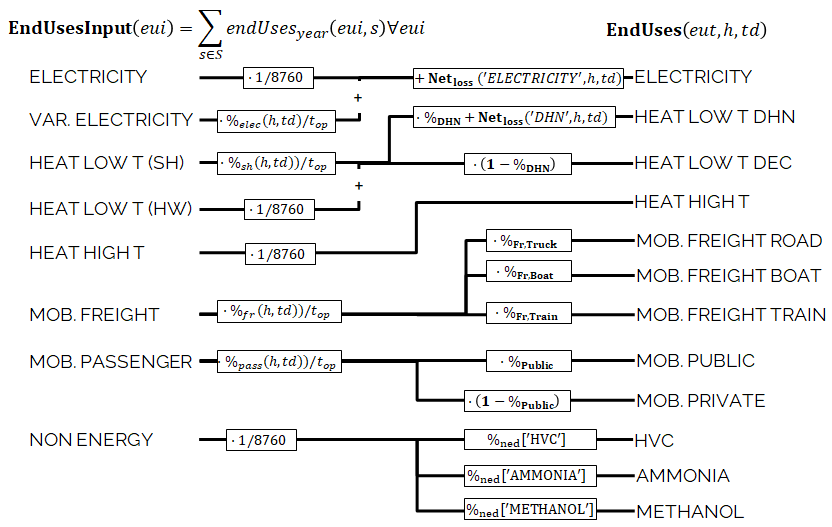
\includegraphics[width=16cm,height=\textheight,keepaspectratio]{/images/model_formulation/EndUseDemand.png}
\caption{Hourly \textbf{EndUses} demands calculation, starting from
yearly demand inputs (\emph{endUsesInput}). Adapted from
Moret2017PhDThesis. This figure was produced for ESTD v2.1. It does not
show the latest EUDs related to cooling and included in v2.2.
Abbreviations: space heating (sh), district heating network (DHN), high
value chemicals (HVC), hot water (HW), passenger (pass), freight (fr)
and non-energy demand (NED).}
\end{figure}

The hourly EUDs (\textbf{EndUses}) are computed based on the yearly EUDs
(\emph{endUsesInput}), distributed according to the time series listed
in
\texttt{Table\ \%s\ \textless{}tab:paramsDistributions\textgreater{}}.
\texttt{Figure\ \%s\ \textless{}fig:EndUseDemand\textgreater{}}
graphically presents the constraints associated to the hourly EUDs
(\textbf{EndUses}). For example, the public mobility demand at time
\(t\) is equal to the hourly passenger mobility demand multiplied by the
public mobility share (\(\textbf{\%}_{\textbf{Public}}
\)).

Electricity EUD results from the sum of the electricity-only demand,
assumed constant throughout the year, and the variable demand for
electricity, distributed across the periods according to \(\%_{elec}\).
Low-temperature heat demand results from the sum of the demand for hot
water (HW), evenly shared across the year, and the demand for space
heating (SH), distributed across the periods according to \(\%_{sh}\).
The percentage repartition between centralized (DHN) and decentralized
heat demand is defined by the variable \(\textbf{\%}_{\textbf{Dhn}}
\). High temperature heat for industrial processes is evenly distributed
across the periods. Passenger mobility demand is expressed in
passenger-kilometers (pkms), while freight demand is in ton-kilometers
(tkms). The variable \(\textbf{\%}_{\textbf{Public}}
\) defines the penetration of public transportation in passenger
mobility. Similarly, \(\textbf{\%}_{\textbf{Rail}}
\), \(\textbf{\%}_{\textbf{Boat}}
\) and \(\textbf{\%}_{\textbf{Truck}}
\) define the penetration of train, boat and trucks for freight
mobility, respectively.

Space cooling demands were added in ESTD v2.2 and are not represented on
\texttt{Figure\ \%s\ \textless{}fig:EndUseDemand\textgreater{}}. The
demand for space cooling (SC) is distributed across the periods
according to \(\%_{sc}\), while the cooling demand for industrial
processes is uniform.

\subsubsection{Cost, emissions and objective
function}\label{cost-emissions-and-objective-function}

{\[\text{min } \textbf{C}_{\textbf{tot}} = \sum_{j \in \text{TECH}} \Big(\textbf{$\tau$}(j) \textbf{C}_{\textbf{inv}}(j) + \textbf{C}_{\textbf{maint}} (j)\Big) + \sum_{i \in \text{RES}} \textbf{C}_{\textbf{op}}(i)\]}

{\[\begin{aligned}
\text{s.t. }  \textbf{$\tau$}(j) =  \frac{i_{\text{rate}}(i_{\text{rate}}+1)^{lifetime(j)}}{(i_{\text{rate}}+1)^{lifetime(j)} - 1} ~~~~~~ \forall j \in \text{TECH}\\
\end{aligned}\]}

{\[\begin{aligned}
\textbf{C}_{\textbf{inv}}(j) = c_{\text{inv}}(j) \textbf{F}(j) ~~~~~~ \forall j \in \text{TECH}\\
\end{aligned}\]}

{\[\begin{aligned}
\textbf{C}_{\textbf{maint}}(j) = c_{\text{maint}}(j) \textbf{F}(j) ~~~~~~ \forall j \in \text{TECH}\\
\end{aligned}\]}

{\[\textbf{C}_{\textbf{op}}(i) = \sum_{t \in T | \{h,td\} \in T\_H\_TD(t)} c_{\text{op}}(i) \textbf{F}_{\textbf{t}}(i,h,td) t_{op} (h,td)  
~~~~~~ \forall i \in \text{RES}\]}

The objective function to minimize is given in
Eq.~\texttt{eq:obj\_func}. It is the the total annual cost of the energy
system (\(\textbf{C}_{\textbf{tot}}\)), defined as the sum of the
annualized investment cost of the technologies
(\(\tau\textbf{C}_{\textbf{inv}}\)), the operating and maintenance costs
of the technologies (\(\textbf{C}_{\textbf{maint}}\)) and the operating
cost of the resources (\(\textbf{C}_{\textbf{op}}\)). The total
investment cost (\(\textbf{C}_{\textbf{inv}}\)) of each technology
results from the multiplication of its specific investment cost
(\(c_{inv}\)) by its installed capacity (\textbf{F})
(Eq.~\texttt{eq:c\_inv}), the latter being defined with respect to the
main end-use output type\footnote{Indeed, some technologies have several
  outputs, such as a CHP. Thus, the installed size must be defined with
  respect to one of these outputs. For example, CHP are defined based on
  the thermal output rather than the electrical one.}.
\(\textbf{C}_{\textbf{inv}}\) is annualised using the factor \(\tau\),
calculated based on the interest rate (\(t_{op}\)) and the technology
lifetime (\emph{lifetime}) in Eq.~\texttt{eq:tau}. The total operation
and maintenance cost is calculated in the same way in
Eq.~\texttt{eq:c\_maint}. In Eq. \texttt{eq:c\_op}, the total cost of
the resources is calculated as the sum of the end-use over different
periods multiplied by the periods\textquotesingle{} duration
(\(t_{op}\)) and the specific cost of the resource (\(c_{op}\)). Note
that in Eq.~\texttt{eq:c\_op}, summing over the typical days using the
set T\phantomsection\label{h_td}{H\_TD}\footnote{To simplify the
  reading, the formulation \(t \in T| \{h,td\} \in T\_H\_TD(t)\) is
  used. However, this cannot be directly implemented in the code and it
  requires two additional sets : \(HOUR\_OF\_PERIOD(t)\) and
  \(TYPICAL\_DAY\_OF\_PERIOD(t)\). Hence, we have:
  \(t \in T| \{h,td\} \in T\_H\_TD(t)\), which is equivalent in the code
  to
  \(t \in T| h \in HOUR\_OF\_PERIOD(t), td \in TYPICAL\_DAY\_OF\_PERIOD(t)\).}
is equivalent to summing over the 8760h of the year.

{\[\textbf{GWP}_\textbf{tot}  = \sum_{j \in \text{TECH}} \frac{\textbf{GWP}_\textbf{constr} (j)}{lifetime(j)} +   \sum_{i \in \text{RES}} \textbf{GWP}_\textbf{op} (i)\]\[\left(\text{in this version of the model} :   \textbf{GWP}_\textbf{tot}  =    \sum_{i \in \text{RES}} \textbf{GWP}_\textbf{op} (i) \right)\]}

{\[\textbf{GWP}_\textbf{constr}(j) = gwp_{\text{constr}}(j) \textbf{F}(j) ~~~~~~ \forall j \in \text{TECH}\]}

{\[\textbf{GWP}_\textbf{op}(i) = \sum_{t \in T| \{h,td\} \in T\_H\_TD(t)} gwp_\text{op}(i) \textbf{F}_\textbf{t}(i,h,td)  t_{op} (h,td )~~~~~~ \forall i \in \text{RES}\]}

The global annual GHG emissions are calculated using a life-cycle
assessment (LCA) approach, i.e. taking into account emissions of the
technologies and resources `\emph{from cradle to grave}'. For climate
change, the natural choice as indicator is the global warming potential
(GWP), expressed in ktCO\(_2\)-eq./year. In Eq.~\texttt{eq:GWP\_tot},
the total yearly emissions of the system
(\(\textbf{GWP}_{\textbf{tot}}\)) are defined as the sum of the
emissions related to the construction and end-of-life of the energy
conversion technologies (\(\textbf{GWP}_{\textbf{constr}}\)), annualized
based on the technology lifetime (\(lifetime\)), and the emissions
related to resources (\(\textbf{GWP}_{\textbf{op}}\)). Similarly to the
costs, the total emissions related to the construction of technologies
are computed in Eq.~\texttt{eq:GWP\_constr} as the product of the
specific emissions (\(gwp_{constr}\)) by the installed capacity
(\(\textbf{F}\)). In Eq.~\texttt{eq:GWP\_op}, the total emissions of the
resources are computed as the emissions associated to fuels from cradle
to combustion and imports of electricity (\(gwp_{op}\)), multiplied by
the period duration (\(t_{op}\)). GWP accounting can be conducted in
different manners depending on the choice of scope. The European
Commission and the IEA mainly use resource-related emissions
(\(\textbf{GWP}_{\textbf{op}}\)) while neglecting indirect emissions
related to the construction of technologies
(\(\textbf{GWP}_{\textbf{constr}}\)). To facilitate the comparison with
their results, a similar implementation is proposed in
Eq.~\texttt{eq:GWP\_tot}.

\subsubsection{System design and
operation}\label{app:sec:system_design_and_operation}

{\[f_{\text{min}} (j) \leq \textbf{F}(j) \leq f_{\text{max}} (j) ~~~~~~ \forall j \in \text{TECH}\]}

Eq.~\texttt{eq:fmin\_fmax} imposes that the installed capacity of a
technology (\textbf{F}) is constrained by upper and lower bounds
(\(f_{max}\) and \(f_{min}\)). This formulation allows for accounting
for old technologies still existing in the target year (lower bound),
but also for the maximum deployment potential of a technology. For
example, regarding offshore wind turbines, (\(f_{min}\)) represents the
existing installed capacity (which will still be available in the near
future), while (\(f_{max}\)) represents the maximum potential.

{\[\textbf{F}_\textbf{t}(i,h,td) \leq \textbf{F}_\textbf{t}(i) \cdot c_{p,t} (i,h,td) ~~~~~~ \forall i \in \text{TECH}, h \in H, td \in TD\]}

{\[\sum_{t \in T| \{h,td\} \in T\_H\_TD(t)} \textbf{F}_\textbf{t}(j,h,td) t_{op}(h,td)  \leq   \textbf{F} (j) c_{p} (j) \sum_{t \in T| \{h,td\} \in T\_H\_TD(t)} t_{op} (h,td)\]\[\forall j \in \text{TECH}\]}

{\[\sum_{t \in T| \{h,td\} \in T\_H\_TD(t)} \textbf{F}_\textbf{t}(i,h,td) t_{op}(h,td)  \leq \text{avail} (i) ~~~~~~ \forall i \in \text{RES}\]}

The operation of resources and technologies in each period is determined
by the decision variable \(\textbf{F}_{\textbf{t}}\). The capacity
factor of technologies is conceptually divided into two components: a
capacity factor for each period (\(c_{p,t}\)) depending on resource
availability (e.g. renewables) and a yearly capacity factor (\(c_{p}\))
accounting for technology downtime and maintenance. For a given
technology, the definition of only one of these two is needed, the other
one being fixed to the default value of 1. For example, intermittent
renewables are constrained by an hourly load factor
(\(c_{p,t}\in[0;1]\)) while CCGTs are constrained by an annual load
factor (\(c_{p}\)) (with a value in that case of 96\% in 2035).
Eqs.~\texttt{eq:cp\_t} and \texttt{eq:c\_p} link the installed size of a
technology to its actual use in each period
(\(\textbf{F}_{\textbf{t}}\)) via the two capacity factors. The total
use of resources is limited by the yearly availability (\(avail\)) in
Eq.~\texttt{eq:res\_avail}.

{\[\sum_{i \in \text{RES}~\cup \text{TECH} \setminus \text{STO}} f(i,l) \textbf{F}_\textbf{t}(i,h,td) + \sum_{j \in \text{STO}} \bigg(\textbf{Sto}_\textbf{out}(j,l,h,td) - \textbf{Sto}_\textbf{in}(j,l,h,td)\bigg)\]\[- \textbf{EndUses}(l,h,td) = 0\]\[\forall l \in L, \forall h \in H, \forall td \in TD\]}

The matrix \(f\) defines, for all technologies and resources, their
output layers (positive) and input layers (negative).
Eq.~\texttt{eq:layer\_balance} expresses the balance for each layer: all
outputs from resources and technologies (including storage) are used to
satisfy the EUDs or as inputs to other resources and technologies.

\subsubsection{Storage}\label{storage}

{\[\textbf{Sto}_\textbf{level} (j,t) =    \textbf{Sto}_\textbf{level} (j,t-1)\cdot\left(1 - \%_{sto_{loss}}(j) \right)\]\[+ t_{op} (h,td)\cdot \Big(\sum_{l \in L | \eta_{\text{sto,in} (j,l) > 0}} \textbf{Sto}_\textbf{in}  (j,l,h,td) \eta_{\text{sto,in}} (j,l)\]\[~~~~~~ - \sum_{l \in L | \eta_{\text{sto,out} (j,l) > 0}} \textbf{Sto}_\textbf{out} (j,l,h,td) /  \eta_{\text{sto,out}} (j,l)\Big)\]\[\forall j \in \text{STO}, \forall t \in \text{T}| \{h,td\} \in T\_H\_TD(t)\]}

{\[\textbf{Sto}_\textbf{level} (j,t) = \textbf{F}_\textbf{t} (j,h,td) ~~~~~~ \forall j \in \text{STO DAILY},\forall t \in \text{T}| \{h,td\} \in T\_H\_TD(t)\]}

{\[\textbf{Sto}_\textbf{level} (j,t) \leq \textbf{F} (j) ~~~~~~ \forall j \in \text{STO} \setminus \text{STO DAILY},\forall t \in \text{T}\]}

In Eq.~\texttt{eq:sto\_level}, the storage level
(\(\textbf{Sto}_{\textbf{level}}\)) at time step \(t\) is defined as the
storage level at \(t-1\) (accounting for the losses in \(t-1\)), plus
the inputs to the storage, minus the output from the storage (accounting
for input/output efficiencies). The storage systems which can only be
used for short-term (daily) applications are included in the daily
storage set (STO DAILY). For these units,
Eq.~\texttt{eq:Sto\_level\_bound\_DAILY}: imposes that the storage level
be the same at the end of each typical day\footnote{In most cases, the
  activation of the constraint stated in Eq. \texttt{eq:sto\_level} will
  have as a consequence that the level of storage be the same at the
  beginning and at the end of each day --- hence the use of the
  terminology `\emph{daily storage}'. Note, however, that such daily
  storage behaviour is not always guaranteed by this constraint and
  thus, depending on the typical days sequence, a daily storage
  behaviour might need to be explicitly enforced.}. Adding this
constraint drastically reduces the computational time. For the other
storage technologies, which can also be used for seasonal storage, the
capacity is bounded by Eq.~\texttt{eq:Sto\_level\_bound}. For these
units, the storage behaviour is thus optimized over 8760 hours.

{\[\textbf{Sto}_\textbf{in}(j,l,h,td)\cdot \Big(\lceil  \eta_{sto,in}(j,l)\rceil -1 \Big) = 0  ~~~~~~ \forall j \in \text{STO},\forall l \in \text{L}, \forall h \in \text{H}, \forall td \in \text{TD}\]}

{\[\textbf{Sto}_\textbf{out}(j,l,h,td)\cdot \Big(\lceil  \eta_{sto,out}(j,l)\rceil -1 \Big) = 0  ~~~~~~ \forall j \in \text{STO},\forall l \in \text{L}, \forall h \in \text{H}, \forall td \in \text{TD}\]}

{\[\Big(\textbf{Sto}_\textbf{in} (j,l,h,td)t_{sto_{in}}(\text{j}) + \textbf{Sto}_\textbf{out}(j,l,h,td)t_{sto_{out}}(\text{j})\Big) \leq \textbf{F} (j)\%_{sto_{avail}}(j)\]\[\forall j \in STO \setminus {V2G} , \forall l \in L, \forall h \in H, \forall td \in TD\]}

Eqs.~\texttt{eq:StoInCeil} - \texttt{eq:StoOutCeil} force the power
input and output to zero if the layer is incompatible\footnote{In the
  code, these equations are implemented with a \emph{if-then} statement.}.
For example, a PHS will only be linked to the electricity layer
(input/output efficiencies \(>\) 0). All other efficiencies will be
equal to 0, to impede that the PHS exchanges with incompatible layers
(e.g. mobility, heat, etc). Eq.~\texttt{eq:LimitChargeAndDischarge}
limits the power input/output of a storage technology based on its
installed capacity (\textbf{F}) and three specific characteristics.
First, storage availability (\(\%_{sto_{avail}}\)) is defined as the
ratio between the available storage capacity and the total installed
capacity (default value is 100\%). This parameter is only used to
realistically represent V2G, for which we assume that only a fraction of
the fleet (i.e. 20\% in these cases) can charge/discharge at the same
time. Second and third, the charging/discharging time (\(t_{sto_{in}}\),
\(t_{sto_{out}}\)), which are the time to complete a full
charge/discharge from empty/full storage\footnote{In this linear
  formulation, storage technologies can charge and discharge at the same
  time. On the one hand, this avoids the need of integer variables; on
  the other hand, it has no physical meaning. However, in a cost
  minimization problem, the cheapest solution identified by the solver
  will always choose to either charge or discharge at any given \(t\),
  as long as cost and efficiencies are defined. Hence, we recommend to
  always verify numerically the fact that only storage inputs or outputs
  are activated at each \(t\), as we do in all our implementations.}.
For example, a daily thermal storage needs at least 4 hours to discharge
(\(t_{sto_{out}}=4\){[}h{]}), and another 4 hours to charge
(\(t_{sto_{in}}=4\){[}h{]}). Eq.~\texttt{eq:LimitChargeAndDischarge}
applies for all storage except electric vehicles which are limited by
another constraint Eq. \texttt{eq:LimitChargeAndDischarge\_ev},
presented later.

\subsubsection{Networks}\label{networks}

{\[\textbf{Net}_\textbf{loss}(eut,h,td) = \Big(\sum_{i \in \text{RES} \cup \text{TECH} \setminus \text{STO} | f(i,eut) > 0} f(i,eut)\textbf{F}_\textbf{t}(i,h,td) \Big) \%_{\text{net}_{loss}} (eut)\]\[\forall eut = \text{EUT}, \forall h \in H, \forall td \in TD\]}

{\[\textbf{F} (Grid) = 1 + \frac{c_{grid,extra}}{c_{inv}(Grid)} 
\Big(
\textbf{F}(Wind_{onshore}) + \textbf{F}(Wind_{offshore}) + \textbf{F}(PV)\]\[-\big( 
f_{min}(Wind_{onshore}) + f_{min}(Wind_{offshore}) + f_{min}(PV)
\big)
\Big)\]}

{\[\textbf{F} (DHN) = \sum_{j \in \text{TECH} \setminus {STO} | f(j,\text{HeatLowTDHN}) >0} f(j,\text{HeatLowTDHN}) \cdot \textbf{F} (j)\]}

{\[\textbf{F} (H_{2,infrastructure}) = \textbf{F} (H_{2,electrolysis})\]}

{\[\textbf{F} (ChargingStations) = \textbf{F} (CAR_{BEV})\]}

Eq.~\texttt{eq:loss} calculates network losses as a share
(\(\%_{\text{net}_{loss}}\)) of the total energy transferred through the
network. As an example, losses in the electricity grid are estimated to
be 4.5\% of the energy transferred in 2015\footnote{This is the ratio
  between the losses in the grid and the total annual electricity
  production in Belgium in 2015 Eurostat2017.}.
Eqs.~\texttt{eq:mult\_grid} - \texttt{eq:DHNCost} define the extra
investment for networks. Integration of intermittent RE implies
additional investment costs for the electricity grid
(\(c_{grid,ewtra}\)). For example, the reinforcement of the electricity
grid is estimated to be 518.5 million USD\textsubscript{2021} per
Gigawatt of intermittent renewable capacity installed (see
\hyperref[ssec:app1_grid:]{Data for the grid} for details).
Eq.~\texttt{eq:DHNCost} links the size of DHN to the total size of the
installed centralized energy conversion technologies. Finally, Eq.
\texttt{eq:h2\_network} links the size of the hydrogen network to the
installed capacity for hydrogen production and
\texttt{eq:charging\_stations} does the same for the infrastructure of
charging stations and electrical vehicles.

\subsubsection{Additional Constraints}\label{additional-constraints}

{\[\textbf{F}_\textbf{t} (Nuclear,h,td) = \textbf{P}_\textbf{Nuclear}  ~~~~~~ \forall h \in H, \forall td \in TD\]}

Nuclear power plants are assumed to have no power variation over the
year, Eq.~\texttt{eq:CstNuke}. If needed, this equation can be
replicated for all other technologies for which a constant operation
over the year is desired.

{\[\textbf{F}_\textbf{t} (j,h,td) = \textbf{\%}_\textbf{PassMob} (j)   \sum_{l \in EUT\_of\_EUC(PassMob)} \textbf{EndUses}(l,h,td)
\]\[\forall j \in TECH\_OF\_EUC(PassMob) , \forall h \in H, \forall td \in TD\]}

{\[\textbf{F}_\textbf{t} (j,h,td) = \textbf{\%}_\textbf{FreightMob} (j)   \sum_{l \in EUT\_of\_EUC(FreightMob)} \textbf{EndUses}(l,h,td)
\]\[\forall j \in TECH\_OF\_EUC(FreightMob) , \forall h \in H, \forall td \in TD\]}

{\[\textbf{\%}_\textbf{Fr,Rail} + \textbf{\%}_\textbf{Fr,Train} + \textbf{\%}_\textbf{Fr,Boat} = 1
\]}

Eqs.~\texttt{eq:mob\_share\_fix} - \texttt{eq:freight\_share\_fix}
impose that the share of the different technologies for mobility
(\(\textbf{\%}_{\textbf{PassMob}}
\)) and (\(\textbf{\%}_{\textbf{Freight}}
\)) be the same at each time step\footnote{{[}foot:nonLinear{]}All
  equations expressed in a compact non-linear form in this section
  Eqs.~\texttt{eq:mob\_share\_fix}, \texttt{eq:freight\_share\_fix},
  \texttt{eq:heat\_decen\_share} and \texttt{eq:dhn\_peak} can be
  linearised. For these cases, the \textbf{EndUses} is defined with
  parameters and a variable representing a constant share over the year
  (e.g. \(\textbf{\%}_\textbf{public}
  \)). As an example, \textbf{EndUses} in
  Eq.~\texttt{eq:mob\_share\_fix} is equal to
  \(\textbf{EndUsesInput}(PassMb) \cdot \%pass (h, td) / t_op (h, td)
  \). The term \(\textbf{\%}_{\textbf{public}}
  \), is missing in the equation, but is implicitly implemented in
  \(\textbf{\%}_{\textbf{PassMob}}
  \).}. In other words, if 20\% of the mobility is supplied by train,
this share remains constant in the morning or the afternoon.
Eq.~\texttt{eq:freight\_share\_constant} verifies that the freight
technologies supply the overall freight demand (this constraint is
related to
\texttt{Figure\ \%s\ \textless{}fig:EndUseDemand\textgreater{}}).

\subsubsection{Decentralised heat
production}\label{decentralised-heat-production}

{\[\textbf{F} (Dec_{Solar}) = \sum_{j \in \text{TECH OF EUT} (\text{HeatLowTDec}) \setminus \{ Dec_{Solar} \}} \textbf{F}_\textbf{sol} (j)\]}

{\[\textbf{F}_{\textbf{t}_\textbf{sol}} (j,h,td) \leq  \textbf{F}_\textbf{sol} (j)  c_{p,t}(Dec_{Solar},h,td)\]\[\forall j \in \text{TECH OF EUT} (\text{HeatLowTDec}) \setminus \{ Dec_{Solar} \}, \forall h\in H, \forall td \in TD\]}

Thermal solar is implemented as a decentralized technology. It is always
installed together with another decentralized technology, which serves
as backup to compensate for the intermittency of solar thermal. Thus, we
define the total installed capacity of solar thermal
\textbf{F}(\(Dec_{solar}\)) as the sum of
\(\textbf{F}_{\textbf{sol}}(j)\),
Eq.~\texttt{eq:de\_strategy\_dec\_total\_ST}, where
\(\textbf{F}_{\textbf{sol}}(j)\) is the solar thermal capacity
associated to the backup technology \(j\).
Eq.~\texttt{eq:op\_strategy\_dec\_total\_ST} links the installed size of
each solar thermal capacity \(\textbf{F}_{\textbf{sol}}(j)\) to its
actual production
\texttt{\textbackslash{}textbf\{F\}\_\{\textbackslash{}textbf\{t\}\_\textbackslash{}textbf\{sol\}\}(j,h,td)}
via the solar capacity factor
(\(c_{solar_{area,rooftop}p,t}(Dec_{solar})\)).

{\[\textbf{F}_\textbf{t} (j,h,td) + \textbf{F}_{\textbf{t}_\textbf{sol}} (j,h,td)\]\[+ \sum_{l \in \text{L}}\Big( \textbf{Sto}_\textbf{out} (i,l,h,td) - \textbf{Sto}_\textbf{in} (i,l,h,td) \Big)\]\[= \textbf{\%}_\textbf{HeatDec}(\text{j}) \textbf{EndUses}(HeatLowT,h,td)
\]\[\forall j \in \text{TECH OF EUT} (\text{HeatLowTDec}) \setminus \{ Dec_{Solar} \},\]\[i \in \text{TS OF DEC TECH}(j)  , \forall h\in H, \forall td \in TD\]}

\begin{figure}
\centering
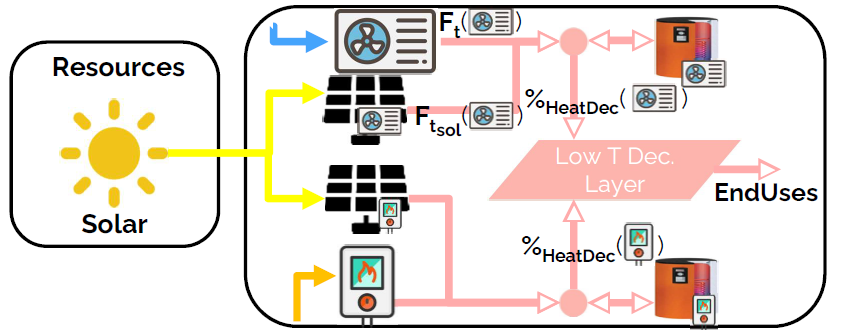
\includegraphics[width=12cm,height=\textheight,keepaspectratio]{/images/model_formulation/ts_and_Fsolv2.png}
\caption{Illustrative example of a decentralised heating layer with
thermal storage, solar thermal and two conventional production
technologies, gas boilers and electrical HP. In this case,
Eq.~\texttt{eq:heat\_decen\_share} applied to the electrical HPs becomes
the equality between the two following terms: left term is the heat
produced by: the eHPs (\(\textbf{F}_{\textbf{t}}(eHPs,h,td)\)), the
solar panel associated to the eHPs
(\(\textbf{F}_{\textbf{t}_\textbf{sol}}(eHPs,h,td)\)) and the storage
associated to the eHPs; right term is the product between the share of
decentralised heat supplied by eHPs
(\(\textbf{\%}_{\textbf{HeatDec}}(eHPs)
\)) and heat low temperature decentralised demand
(\(\textbf{EndUses}(HeatLowT,h,td)\)).}
\end{figure}

A thermal storage \(i\) is defined for each decentralised heating
technology \(j\), to which it is related via the set \emph{TS OF DEC
TECH}, i.e. \(i\)=*TS OF DEC TECH(j)*. Each thermal storage \(i\) can
store heat from its technology \(j\) and the associated thermal solar
\(\textbf{F}_{\textbf{sol}}\) (\(j\)). Similarly to the passenger
mobility, Eq.~\texttt{eq:heat\_decen\_share} makes the model more
realistic by defining the operating strategy for decentralized heating.
In fact, in the model we represent decentralized heat in an aggregated
form; however, in a real case, residential heat cannot be aggregated. A
house heated by a decentralised gas boiler and solar thermal panels
should not be able to be heated by the electrical heat pump and thermal
storage of the neighbours, and vice-versa. Hence,
Eq.~\texttt{eq:heat\_decen\_share} imposes that the use of each
technology (\(\textbf{F}_{\textbf{t}}(j,h,td)\)), plus its associated
thermal solar (\(\textbf{F}_{\textbf{t}_\textbf{sol}}(j,h,td)\)) plus
its associated storage outputs
(\(\textbf{Sto}_{\textbf{out}}(i,l,h,td)\)) minus its associated storage
inputs (\(\textbf{Sto}_{\textbf{in}}(i,l,h,td)\)) should be a constant
share (\(\textbf{\%}_{\textbf{HeatDec}}(j)
\)) of the decentralised heat demand
\((\textbf{EndUses}(HeatLowT,h,td)\)).
\texttt{Figure\ \%s\ \textless{}fig:FsolAndTSImplementation\textgreater{}}
shows, through an example with two technologies (a gas boiler and a HP),
how decentralised thermal storage and thermal solar are implemented.

\subsubsection{Vehicle-to-grid}\label{vehicle-to-grid}

\begin{figure}
\centering
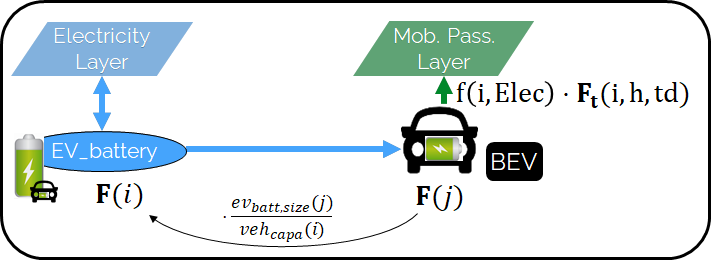
\includegraphics[width=7cm,height=\textheight,keepaspectratio]{/images/model_formulation/v2gAndBatteries.png}
\caption{Illustrative example of a V2G implementation. The battery can
interact with the electricity layer. The size of the battery is directly
related to the number of cars (see Eq. \texttt{eq:SizeOfBEV}). The V2G
takes the electricity from the battery to provide a constant share
(\(\textbf{\%}_{\textbf{PassMob}}
\)) of the passenger mobility layer (\emph{Mob. Pass.}). Thus, it
imposes the amount of electricity that electric car must deserve (see
Eq. \texttt{eq:BtoBEV}). The remaining capacity of battery available can
be used to provide V2G services (see
\texttt{eq:LimitChargeAndDischarge\_ev}).}
\end{figure}

{\[\textbf{F} (i) = \frac{\textbf{F} (j)}{ veh_{capa} (j)} ev_{batt,size} (j)  ~~~~~~ \forall  j \in  V2G, i \in \text{EVs_BATT OF V2G}(j)\]}

Vehicle-to-grid dynamics are included in the model via the \emph{V2G}
set. For each vehicle \(j \in V2G\), a battery \(i\) (\(i\) \(\in\)
\emph{EVs\_BATT}) is associated using the set
EVs\phantomsection\label{batt_of_v2g}{BATT\_OF\_V2G}
(\(i \in \text{EVs_BATT_OF_V2G}(j)\)). Each type \(j\) of \emph{V2G} has
a different size of battery per car (\(ev_{batt,size}(j)\)), e.g. the
first generation battery of the Nissan Leaf (ZE0) has a capacity of 24
kWh\footnote{This generation (ZE0) was marketed from 2010 to 2017 with a
  battery capacity of 24~kWh. The new generation (ZE1) accounts for an
  improved capacity and reaches 40~kWh per battery. Data from
  \url{https://en.wikipedia.org/wiki/Nissan_Leaf}, consulted on
  08-02-2021}. The number of vehicles of a given technology is
calculated with the installed capacity (\textbf{F}) in {[}km-pass/h{]}
and its capacity per vehicles (\(veh_{capa}\) in {[}km-pass/h/veh.{]}).
Thus, the energy that can be stored in batteries \textbf{F}(\(i\)) of
\emph{V2G}(\(j\)) is the ratio of the installed capacity of vehicle by
its specific capacity per vehicles times the size of battery per car
(\(ev_{batt,size}(j)\)), Eq.~ \texttt{eq:SizeOfBEV}. For example, if
this technology of cars covers 10 Mpass-km/h, and the capacity per
vehicle is 50.4 pass-km/car/h (which represents an average speed of
40km/h and occupancy of 1.26 passenger per car); thus, the amount of BEV
cars are 0.198 million cars. And if a BEV has a 24kWh of battery, such
as the Nissan Leaf (ZE0), thus, the equivalent battery has a capacity of
4.76 GWh.

{\[\textbf{Sto}_\textbf{out} (j,Elec,h,td) \geq - f(i,Elec) \textbf{F}_\textbf{t} (i,h,td)\]\[\forall i \in V2G , \forall j \in \text{EVs_BATT OF V2G}(j), \forall h \in H, td \in TD\]}

Eq.~\texttt{eq:BtoBEV} forces batteries of electric vehicles to supply,
at least, the energy required by each associated electric vehicle
technology. This lower bound is not an equality; in fact, according to
the V2G concept, batteries can also be used to support the grid.
\texttt{Figure\ \%s\ \textless{}fig:V2GAndBatteries\textgreater{}} shows
through an example with only BEVs how Eq.~\texttt{eq:BtoBEV} simplifies
the implementation of V2G. In this illustration, a battery technology is
associated to a BEV. The battery can either supply the BEV needs or
sends electricity back to the grid.

{\[\textbf{Sto}_\textbf{in} (j,l,h,td)t_{sto_{in}}(\text{j}) + \Big(\textbf{Sto}_\textbf{out}(j,l,h,td) + f(i,Elec) \textbf{F}_\textbf{t} (i,h,td) \Big) \cdot t_{sto_{out}}(\text{j})\]\[\leq \Big( \textbf{F} (j) - \frac{\textbf{F} (j)}{ veh_{capa} (j)} ev_{batt,size} (j) \Big) \cdot \%_{sto_{avail}}(j)\]\[\forall i \in V2G , \forall j \in \text{EVs\_BATT OF V2G}(j) , \forall l \in L, \forall h \in H, \forall td \in TD\]}

Eq.~\texttt{eq:LimitChargeAndDischarge\_ev} limits the availability of
batteries to the number of vehicle connected to the grid. This equation
is similar to the one for other type of storage (see Eq.
\texttt{eq:LimitChargeAndDischarge}); except that a part of the
batteries are not accounted, i.e. the one running (see Eq.
\texttt{eq:BtoBEV}). Therefore, the available output is corrected by
removing the electricity powering the running car (here,
\(f(i,Elec) \leq 0\)) and the available batteries is corrected by
removing the numbers of electric cars running
(\(\frac{\textbf{F} (j)}{ veh_{capa} (j)} ev_{batt,size} (j)\)).

{\[\textbf{Sto}_\textbf{level} (j,t) \geq \textbf{F}[i] soc_{ev}(i,h)\]\[\forall i \in V2G , \forall j \in \text{EVs\_BATT OF V2G}(j) , \forall t \in T| \{h,td\} \in T\_H\_TD\]}

For each electric vehicle (\(ev\)), a minimum state of charge is imposed
for each hour of the day big(\(soc_{ev}(i,h)\)big). For example, we can
impose that the state of charge of EV is 60\% in the morning, to ensure
that cars can be used to go for work.
Eq.~\texttt{eq:EV\_min\_state\_of\_charge} imposes, for each type of
{V2G}, that the level of charge of the EV batteries is greater than the
minimum state of charge times the storage capacity.

\subsubsection{Peak demand}\label{peak-demand}

{\[\textbf{F} (j) 
\geq
\%_{Peak_{sh}}\max_{h\in H,td\in TD}\left\{\textbf{F}_\textbf{t}(j,h,td)\right\}\]\[\forall j \in \text{TECH OF  EUT} (HeatLowTDEC)   \setminus \{ Dec_{Solar}\}\]}

{\[\sum_{\hspace{3cm}j \in \text{TECH OF EUT} (HeatLowTDHN), i \in \text{STO OF EUT}(HeatLowTDHN)}\]\[\Big( \textbf{F} (j)+
\textbf{F} (i)/t_{sto_{out}}(i,HeatLowTDHN)  \Big)\]\[\geq
\%_{Peak_{sh}} \max_{h\in H,td\in TD}  \big\{ \textbf{EndUses}(HeatLowTDHN,h,td) \big\}\]}

{\[\textbf{F} (j) 
\geq
\%_{Peak_{sc}}\max_{h\in H,td\in TD}\left\{\textbf{F}_\textbf{t}(j,h,td)\right\}\]\[\forall j \in \text{TECH OF  EUT} (SpaceCooling)\]}

Finally, Eqs.~\texttt{eq:dec\_peak} - \texttt{eq:dhn\_peak} constrain
the installed capacity of low temperature heat supply. Based on the
selected TDs, the ratio between the yearly peak demand and the TDs peak
demand is defined for space heating (\(\%_{Peak_{sh}}\)).
Eq.~\texttt{eq:dec\_peak} imposes that the installed capacity for
decentralised technologies covers the real peak over the year.
Similarly, Eq.~\texttt{eq:dhn\_peak} forces the centralised heating
system to have a supply capacity (production plus storage) higher than
the peak demand. These equations force the installed capacity to meet
the peak heating demand, i.e. which represents, somehow, the network
adequacy\footnote{The model resolution of the dispatch is not accurate
  enough to verify the adequacy. As one model cannot address all the
  issues, another approach has been preferred: couple the model to a
  dispatch one, and iterate between them. Percy and Coates
  percy\_coates\_coupling\_2020 demonstrated the feasibility of coupling
  a design model (ESTD) with a dispatch one (Dispa-SET Quoilin2017).
  Based on a feedback loop, they iterated on the design to verify the
  power grid adequacy and the strategic reserves. Results show that the
  backup capacities and storage needed to be slightly increased compared
  to the results of the design model alone.}. Similarly to
\texttt{eq:dec\_peak}, \texttt{eq:sc\_peak} imposes that the installed
capacity for space cooling technologies covers the real peak cooling
demand over the year.

\subsubsection{Adaptations for the case
study}\label{sssec_lp_adaptation_case_study}

Additional constraints are required to implement scenarios. Scenarios
require six additional constraints (Eqs.~\texttt{eq:LimitGWP} -
\texttt{eq:solarAreaLandLimited}) to impose a limit on the GWP
emissions, the minimum share of RE primary energy, the relative shares
of technologies, such as gasoline cars in the private mobility, the cost
of energy efficiency measures, the electricity import power capacity and
the available surface area for solar technologies.

{\[\textbf{GWP}_\textbf{tot} \leq gwp_{limit}\]}

{\[\sum_{j \in  \text{RES}_\text{re},t \in T| \{h,td\} \in T\_H\_TD(t)} \textbf{F}_\textbf{t}(j,h,td)  \cdot  t_{op} (h,td)\]\[\geq 
re_{share} \sum_{j \in \text{RES} ,t \in T| \{h,td\} \in T\_H\_TD(t)} \textbf{F}_\textbf{t}(j,h,td) \cdot  t_{op} (h,td)\]}

To force the energy system to decrease its emissions, two lever can
constraint the annual emissions: Eq.~\texttt{eq:LimitGWP} imposes a
maximum yearly emissions threshold on the GWP (\(gwp_{limit}\)); and
Eq.~\texttt{eq:LimitRE} fixes the minimum renewable primary energy
share.

{\[f_{\text{min,\%}}(j) \sum_{j' \in \text{TECH OF EUT} (eut),t \in T|\{h,td\} \in T\_H\_TD(t)}    \textbf{F}_\textbf{t}(j',h,td)\cdot t_{op}(h,td)
\]\[\leq 
\sum_{t \in T|\{h,td\} \in T\_H\_TD(t)}  \textbf{F}_\textbf{t} (j,h,td)\cdot t_{op}(h,td)\]\[\leq 
f_{\text{max,\%}}(j) \sum_{j'' \in \text{TECH OF EUT} (eut),t \in T|\{h,td\} \in T\_H\_TD(t)}    \textbf{F}_\textbf{t}(j'',h,td)\cdot t_{op}(h,td)
\]\[\forall eut \in EUT, \forall j \in \text{TECH OF EUT} (eut)\]}

To represent the national energy system under study,
Eq.~\texttt{eq:fmin\_max\_perc} imposes the relative share of a
technology in its sector. Eq.~\texttt{eq:fmin\_max\_perc} is
complementary to Eq.~\texttt{eq:fmin\_fmax}, as it expresses the minimum
(\(f_{min,\%}\)) and maximum (\(f_{max,\%}\)) yearly output shares of
each technology for each type of EUD. In fact, for a given technology,
assigning a relative share (e.g. boilers providing at least a given
percentage of the total heat demand) is more intuitive and close to the
energy planning practice than limiting its installed size.
\(f_{min,\%}\) and \(f_{max,\%}\) are fixed to 0 and 1, respectively,
unless otherwise indicated.

{\[\begin{aligned}
\sum_{t \in T|\{h,td\} \in T\_H\_TD(t)} \big(\textbf{F}_\textbf{t}(Motorcycle,h,td)
+ \textbf{F}_\textbf{t}(Motorcycle~Electric,h,td)\big) \cdot t_{op}(h,td) \\
\leq \%_{max,motorcycle}~\sum_{j \in \text{TECH OF EUT} (Mob~Private), t \in T|\{h,td\} \in T\_H\_TD(t)} \textbf{F}_\textbf{t}(j,h,td)\cdot t_{op}(h,td)
\end{aligned}\]}

Similarly to eq. \texttt{eq:fmin\_max\_perc}, eq.
\texttt{eq:f\_max\_perc\_motorcycle} imposes the maximum share of
private passenger mobility that can be supplied by motorcycles.

{\[\textbf{F}(Efficiency) =  \frac{1}{1+i_{rate}}\]}

Eq.~\texttt{eq:efficiency} is supposed to compute the cost of efficiency
measures. This equation was used to put a cost on the energy efficiency
measures envisaged by the EU Commission for European countries. It is
not used for the case of Colombia and Turkey (i.e. F(Efficiency) is
multiplied by a zero-cost later on).

\subsubsection{Additional contraints on imports, exports and
renewables}\label{sssec_lp_imports_exports_renewables}

{\[\textbf{F}_{\textbf{t}}(Electricity,h,td) \leq  elec_{import,max} + \textbf{F}(HVAC~Line) ~~~~~~ \forall h \in H, \forall td \in TD\]}

{\[\textbf{F}_{\textbf{t}}(Elec~Export,h,td) \leq  elec_{export,max} + \textbf{F}(HVAC~Line) ~~~~~~ \forall h \in H, \forall td \in TD\]}

{\[\textbf{F}_{\textbf{t}}(i,h,td) \cdot t_{op} (h,td) =  \textbf{Import}_{\textbf{constant}}(i) ~~~~~~ \forall i \in \text{RES~IMPORT~CONSTANT}, h \in H, td \in TD\]}

{\[\textbf{F}_{\textbf{t}}(i,h,td) \cdot t_{op} (h,td) =  \textbf{Export}_{\textbf{constant}}(i) ~~~~~~ \forall i \in \text{EXPORT~E~FUEL}, h \in H, td \in TD\]}

Eqs.~\texttt{eq:elecImpLimited} and \texttt{eq:elecExpLimited} limit the
power grid import and export capacity from/to neighbouring countries,
based on the 2021 import/export capacity plus the construction of new
High-Voltage transfer capacity (HVAC Line).
Eq.~\texttt{eq:import\_resources\_constant} imposes that some resources
are imported at a constant power. For example, gas and hydrogen are
supposed to be imported at a constant flow during the year. In addition
to offering a more realistic representation, this implementation makes
it possible to visualise the level of storage within the region.
Eq.~\texttt{eq:export\_efuels\_constant} imposes the same constraint as
\texttt{eq:import\_resources\_constant}, but for the \emph{export} of
e-fuels.

Caution

Adding too many ressource to Eq. \texttt{eq:import\_resources\_constant}
increases drastically the computational time. In this implementation,
only resources expensive to store have been accounted for i.e. hydrogen
and gas. Other resources, such as diesel or ammonia, can be stored at a
cheap price with small losses. By limiting EXPORT-E-FUEL to two types of
resources (hydrogen and gas), the computation time is below a minute.
When adding all imported resources to EXPORT-E-FUEL, the computational
time becomes above 6 minutes.

{\[\frac{\textbf{F}(Dam~Storage) - f_{min}(Dam~Storage)}{f_{max}(Dam~Storage) - f_{min}(Dam~Storage)} \leq \frac{\textbf{F}(Hydro~Dam) - f_{min}(Hydro~Dam)}{f_{max}(Hydro~Dam) - f_{min}(Hydro~Dam)}\]}

{\[\textbf{Sto}_\textbf{in}(Dam~Storage,Electricity,h,td) = \textbf{F}_{\textbf{t}}(Hydro~Dam,h,td) ~~~~~~ \forall h \in H, \forall td \in TD\]}

{\[\textbf{Sto}_\textbf{out}(Dam~Storage,Electricity,h,td) \leq \textbf{F}(Hydro~Dam,h,td) ~~~~~~ \forall h \in H, \forall td \in TD\]}

In EnergyScope, there are two technologies related to hydro-electric
dams: \emph{Hydro Dam} and \emph{Dam Storage}. The former relates to the
electricity production function of hydro-electric dams, while the second
relates to their storage function. These two functions are defined as
separate technologies in EnergyScope, but of course they relate to the
same physical asset. The constraints defined in eqs
\texttt{eq:link\_dam\_storage\_to\_hydro\_dam} -
\texttt{eq:dam\_storage\_out} hence bind these two technologies to each
other. First, eq. \texttt{eq:link\_dam\_storage\_to\_hydro\_dam} imposes
that the installed capacity of both technnologies must remain
proportional to each other, in the proportions defined by their
respective input parameters \(f_{min}\) and \(f_{max}\). (Note that to
improve readability, eq. \texttt{eq:link\_dam\_storage\_to\_hydro\_dam}
has been written in a non-linear fashion in this documentation. The
equation is linear in the actual model\textquotesingle s code). Second,
eq. \texttt{eq:dam\_storage\_in} imposes that all electricity produced
by \emph{Hydro Dam} is immediately absorbed by \emph{Dam Storage}. This
electricity is then released by \emph{Dam Storage}, under the constraint
that the maximum electricity production of \emph{Dam Storage} is the
same one as for \emph{Hydro Dam}.

{\[-\frac{\textbf{F}(ST~Collector)}{f(ST~Power~Block, ST~Heat)} \leq sm_{max} \cdot \textbf{F}(ST~Power~Block)\]}

{\[-\frac{\textbf{F}(PT~Collector)}{f(PT~Power~Block, PT~Heat)} \leq sm_{max} \cdot \textbf{F}(PT~Power~Block)\]}

Concentrated solar power (CSP) technologies are modelled with 3
elements: \emph{Collectors}, \emph{Storage} and \emph{Power Block}. The
link between the 3 elements is kept into a "realistic" range thanks to
Equations \texttt{eq:limit\_solar\_mulitple\_ST} and
\texttt{eq:limit\_solar\_mulitple\_PT}.

{\[\frac{\textbf{F}(PV~Rooftop)}{power\_density_{pv}} + \frac{\textbf{F}(Dec_{Solar}) + \textbf{F}(DHN_{Solar})}{power\_density_{solar~thermal}}  \leq solar_{area,rooftop}\]}

{\[\begin{aligned}
\frac{\textbf{F}(PV~Utility)}{power\_density_{pv}} - \frac{\textbf{F}(ST~Collector)}{f(ST~Power~Block, ST~Heat) \cdot power\_density_{csp}}\\
- \frac{\textbf{F}(PT~Collector)}{f(PT~Power~Block, PT~Heat) \cdot power\_density_{csp}}\leq solar_{area,ground}
\end{aligned}\]}

{\[\begin{aligned}
- \frac{\textbf{F}(ST~Collector)}{f(ST~Power~Block, ST~Heat)\cdot power\_density_{csp}}\\
- \frac{\textbf{F}(PT~Collector)}{f(PT~Power~Block, PT~Heat) \cdot power\_density_{csp}}  \leq solar_{area,ground,high~irr}
\end{aligned}\]}

In this version of EnergyScope, the upper limit for the deployment of
solar technologies is calculated based on the available areas
(\(solar_{area}\)) and power densities (\(power\_density\)) of solar
technologies. The conversion factor between an installed capacity (in
watt peak (Wp)) and the surface used (in \(km^2\)) is calculated based
on the peak power density (in {[}Wp/m\(^2\){]}). Put simply, the peak
power density represents the peak power of one square meter of solar
panel. Thus, the land use of a solar technology is its installed
capacity (\(\textbf{F}(\cdot)\), in {[}GW{]}) divided by its power peak
density (in {[}GW/km\(^2\){]}). Eq. \texttt{eq:solarAreaRooftopLimited}
imposes a constraint on the available rooftop area for solar energy. Eq.
\texttt{eq:solarAreaLandLimited}, does the same for ground area.
Finally, eq. \texttt{eq:solarAreaGroundHighIrrLimited} proceeds
similarly for ground area with high irradiation, suitable for the
installation of CSP plants (i.e. with a Direct Normal Irradiation (DNI)
superior to 1800 {[}kWh/m\(^2\)/year{]}). The area limitation is applied
on the \emph{Collector} element of the CSP. The capacity of the
\emph{Collector} (which produces heat) is then transformed into the
equivalent electrical power capacity in eqs
\texttt{eq:solarAreaLandLimited} -
\texttt{eq:solarAreaGroundHighIrrLimited}, using the heat-electricity
conversion efficiency of the \emph{Power block}. Indeed, the
\(power\_density_{csp}\) is expressed in electrical GW, not in thermal
GW. Note that in eqs. \texttt{eq:solarAreaLandLimited} -
\texttt{eq:solarAreaGroundHighIrrLimited}, the terms associated with CSP
are counted as positive (the minus signs are present to compensate for
the negative signs of \(f(\cdot)\)).

\section{Implementation}\label{ssec_estd_implementation}

The implementation into code of the MILP and LP problems has been
carried out using an algebraic modelling language. Such modelling
language allows for the representation of large LP and MILP problems.
Its syntax is similar to AMPL, which is -according to the
NEOS-statistics\footnote{NEOS Server is an Internet-based client-server
  application that provides free access to a library of optimization
  solvers. Statistics are available at:
  \url{https://neos-server.org/neos/report.html}, consulted the
  27/01/2021.} - the most popular format for representing mathematical
programming problems. The chosen formulation enables the use of
different solvers, be it open source ones (e.g. GLPK) or commercial ones
(e.g. CPLEX, Gurobi). Each of the equations defined in this
documentation is found in identical form in the code, together with the
corresponding numbering. SETS, Variables and parameters have the same
names (unless explicitly stated in the definition of the term).
\texttt{Figure\ \%s\ \textless{}fig:ch2\_LP\_formulation\_implementation\_colored\textgreater{}}
illustrates, for the balance constraint \texttt{eq:layer\_balance}, the
mathematical formulation presented in this work and its implementation
in the code. Colors highlight corresponding elements. In the code, each
constraint has a comment (starting with \#) and a name (colored in
black), in this case \emph{layer\_balance}. In addition, most of the
SETS, Variables and parameters are more explicitly named in the code.
For example, the set "layers" is named \emph{L} in the documentation and
\emph{LAYERS} in the code; similarly, the input efficiency is named
\emph{f} in the documentation and \emph{layers\_in\_out} in the code.

\begin{figure}
\centering
\pandocbounded{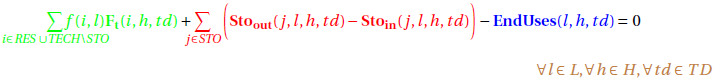
\includegraphics[keepaspectratio]{/images/model_formulation/eqs_color.png}}
\caption{}
\end{figure}

\begin{figure}
\centering
\pandocbounded{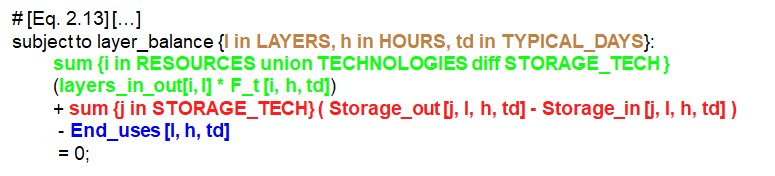
\includegraphics[keepaspectratio]{/images/model_formulation/ch_estd_code_screenshot.png}}
\caption{Comparison of equations\textquotesingle{} formulation in this
documentation (upper) and in the code (lower). Example based on Eq.
\texttt{eq:layer\_balance}.}
\end{figure}

The entire implementation is available on the directory
ESTD\_v2\_1\_repo (standard model for Belgium) and ESTD\_v2\_1\_repo2
(model with python wrapper applied to Colombia and Turkey). In the case
of the model applied to Colombia and Turkey, the directory contains 4
main folders:

\begin{itemize}
\item
  \textquotesingle energyscope\textquotesingle{} contains the code
  describing the model formulation. In particular, all equations
  described above are written as is in the sub-folder
  \textquotesingle energy\phantomsection\label{model}{model}\textquotesingle,
  in the file
  \textquotesingle es\phantomsection\label{model.mod}{model.mod}\textquotesingle.
\item
  \textquotesingle Data\textquotesingle{} contains several data sets in
  different sub-folders, each corresponding to a different case study.
  For example, \textquotesingle CO 2035\textquotesingle{} contains the
  values of all parameters for applying the model to Colombia in the
  year 2035.
\item
  \textquotesingle case\phantomsection\label{studies}{studies}\textquotesingle{}
  contains the ready-to-run AMPL formulation of the model as well as the
  ouptuts of the runs for each case study, in different sub-folders.
\item
  \textquotesingle scripts\textquotesingle{} contains two important
  files:

  \begin{quote}
  \begin{itemize}
  \tightlist
  \item
    config\phantomsection\label{ref.yaml}{ref.yaml} indicates which case
    study is chosen, by pointing towards the right subfolders in
    \textquotesingle Data\textquotesingle{} and
    \textquotesingle case\phantomsection\label{studies}{studies}\textquotesingle{}
    and by indicating the chosen limit for GHG emissions.
  \item
    run\phantomsection\label{energyscope.py}{energyscope.py} is the
    python file which runs everything.
  \end{itemize}
  \end{quote}
\end{itemize}

\phantomsection\label{citations}
\begin{description}
\item[\phantomsection\label{a}{a}]
Generally {[}GWh/y{]}, but {[}Mpkm{]} (millions of passenger-km) for
passenger mobility EUD and {[}Mtkm{]} (millions of ton-km) for freight
mobility EUD
\item[\phantomsection\label{b}{b}]
GWh instead of GW if \({{tech}} \in {{STO}}\)
\item[\phantomsection\label{c}{c}]
{[}Mpkm/h{]} for passenger mobility EUD, {[}Mtkm/h{]} for freight
mobility EUD
\item[\phantomsection\label{d}{d}]
{[}Mpkm{]} (millions of passenger-km) for passenger mobility EUD,
{[}Mtkm{]} (millions of ton-km) for freight EUD
\item[\phantomsection\label{e}{e}]
{[}Mpkm{]} (millions of passenger-km) for passenger mobility EUD,
{[}Mtkm{]} (millions of ton-km) for freight EUD
\end{description}

\end{document}
